\documentclass{sig-alternate}

\newcommand{\TITLE}{Towards a Scientific Impact Measuring Framework for Large Computing Facilities - a Case Study on XSEDE}
\newcommand{\AUTHOR}{Fugang Wang, Gregor von Laszewski}

%%%%%%%%%%%%%%%%%%%%%%%%%%%%%%%%%%%%%%%%%%%%%%%%%%%%%%%%%%%%%%%%%%%%%%
% LATEX DEFINITIONS
%%%%%%%%%%%%%%%%%%%%%%%%%%%%%%%%%%%%%%%%%%%%%%%%%%%%%%%%%%%%%%%%%%%%%%

\usepackage{hyperref}
\usepackage{array}
\usepackage{graphicx}
\usepackage{booktabs}
\usepackage{pifont}
\usepackage{todonotes}
\usepackage{rotating}
\usepackage{color}

\newcommand*\rot{\rotatebox{90}}

\newcommand{\FILE}[1]{\todo[color=green!40]{#1}}

%%%%%%%%%%%%%%%%%%%%%%%%%%%%%%%%%%%%%%%%%%%%%%%%%%%%%%%%%%%%%%%%%%%%%%
% HYPERSETUP
%%%%%%%%%%%%%%%%%%%%%%%%%%%%%%%%%%%%%%%%%%%%%%%%%%%%%%%%%%%%%%%%%%%%%%
\hypersetup{
    bookmarks=true,         % show bookmarks bar?
    unicode=false,          % non-Latin characters in Acrobat’s bookmarks
    pdftoolbar=true,        % show Acrobat’s toolbar?
    pdfmenubar=true,        % show Acrobat’s menu?
    pdffitwindow=false,     % window fit to page when opened
    pdfstartview={FitH},    % fits the width of the page to the window
    pdftitle={\TITLE},    % title
    pdfauthor={\AUTHOR},     % author
    pdfsubject={Subject},   % subject of the document
    pdfcreator={Gregor von Laszewski, Fugang Wang},   % creator of the document
    pdfproducer={Gregor von Laszewski}, % producer of the document
    pdfkeywords={hindex} {metric}{XSEDE} {FutureGrid}, % list of keywords
    pdfnewwindow=true,      % links in new window
    colorlinks=false,       % false: boxed links; true: colored links
    linkcolor=red,          % color of internal links (change box color with linkbordercolor)
    citecolor=green,        % color of links to bibliography
    filecolor=magenta,      % color of file links
    urlcolor=cyan           % color of external links
}

%%%%%%%%%%%%%%%%%%%%%%%%%%%%%%%%%%%%%%%%%%%%%%%%%%%%%%%%%%%%%%%%%%%%%%

\begin{document}
%
% --- Author Metadata here ---
\conferenceinfo{XSEDE}{'14 Atlanta, Georgia, U.S.A.}
\CopyrightYear{2014} 
\crdata{X-XXXXX-XX-X/XX/XX}  % Allows default copyright data (0-89791-88-6/97/05) to be over-ridden - IF NEED BE.
% --- End of Author Metadata ---

\title{\TITLE}
%\subtitle{[Extended Abstract]
%\titlenote{A full version of this paper is available as
%\texttt{www.acm.org/eaddress.htm}}}

\numberofauthors{4} 
\author{
\alignauthor
Fugang Wang\\
       \affaddr{Indiana University}\\
       \affaddr{2719 10th Street}\\
       \affaddr{Bloomington, Indiana, U.S.A.}\\
 % 2nd. author
\alignauthor
Gregor von Laszewski\titlenote{Corresponding Author.}\\
       \affaddr{Indiana University}\\
       \affaddr{2719 10th Street}\\
       \affaddr{Bloomington, Indiana, U.S.A.}\\
       \email{laszewski@gmail.com}
% 3rd. author
\alignauthor
Geoffrey C. Fox\\
       \affaddr{Indiana University}\\
       \affaddr{2719 10th Street}\\
       \affaddr{Bloomington, Indiana, U.S.A.}\\
\and  % use '\and' if you need 'another row' of author names
% 4th. author
\alignauthor 
Tom Furlani\\
       \affaddr{CCR}\\
       \affaddr{Street}\\
       \affaddr{Buffalo NY, 47401}
}
\date{13 March 2014}

\toappear{}
\maketitle
\begin{abstract}

In this paper we presented a framework that does publication and citation data retrieval, scientific impact metrics generation on different aggregated levels, as well as correlation analysis of the impact metrics vs the resource allocation for a computing facility. We applied the framework to conduct scientific impact metrics evaluation of XSEDE, and did extensive statistical analysis on the impact metrics on project level and Field of Science (FOS) level correlating to the Service Units (SUs) allocated by XSEDE. This not only shows the impact of the XSEDE in general, but also details how the impact is reflected on project level and different FOS. Some of the work could be utilized by XSEDE resource allocation review to help achieve higher scientific impact of XSEDE and better return of investment in general.

\end{abstract}

% A category with the (minimum) three required fields
\category{H.4}{Information Systems Applications}{Miscellaneous}
%A category including the fourth, optional field follows...
\category{D.2.8}{Software Engineering}{Metrics}[complexity measures, performance measures]

\terms{Theory}

\keywords{Scientific impact, bibliometric, h-index, Technology audit, XSEDE}

%%%%%%%%%%%%%%%%%%%%%%%%%%%%%%%%%%%%%%%%%%%%%%%%%%%%%%%%%%%%%%%%%%%%%%
% SECTIONS
%%%%%%%%%%%%%%%%%%%%%%%%%%%%%%%%%%%%%%%%%%%%%%%%%%%%%%%%%%%%%%%%%%%%%%

\section{Introduction}


\section{Related}
%\section{Influence from FutureGrid}

Initialy designed by von Laszewski and Wang

drupal

drupal bibliography module

doi numbers

my pupblications

association with projects

report

processes

upload individually

upload as project

upload en mass

vetting

simplified input

``just a text string''
\cite{drupal-bib}





%\section{requirements}

\section{design.tex}



\begin{figure}[htb]
  \centering
    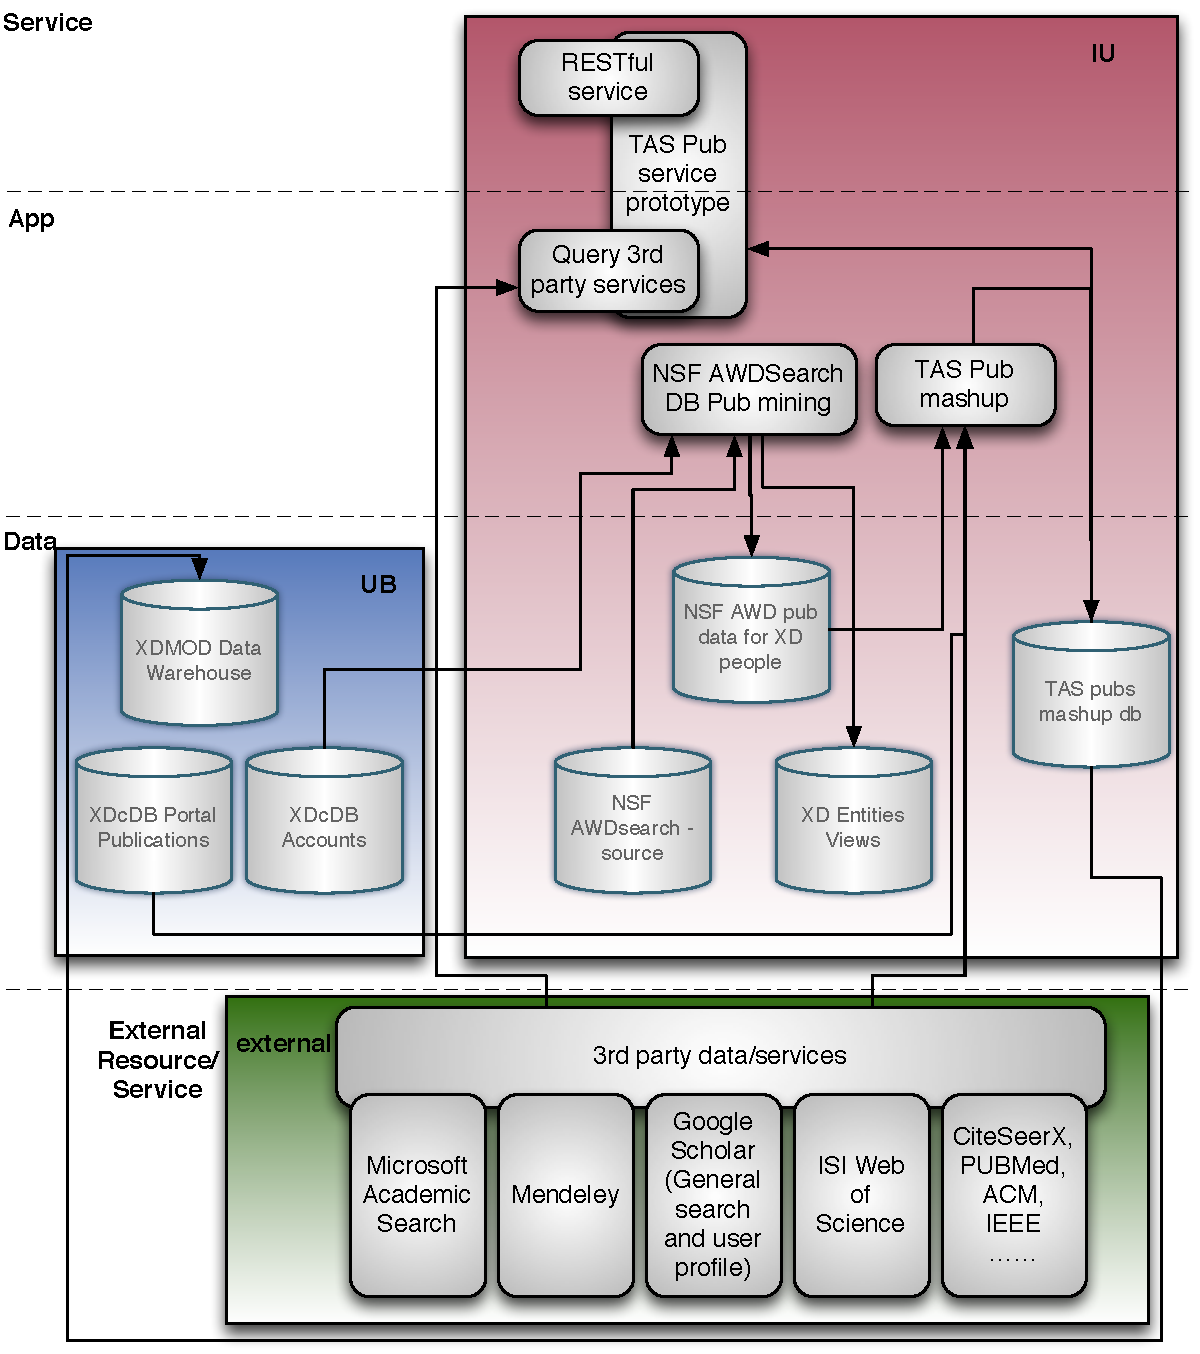
\includegraphics[width=1.0\columnwidth]{images/tas-arch.pdf}
  \caption{tas-arch.}\label{F:tas-arch}
\end{figure}



\section{Implementation}

We have implemented the system following best practices and leveraging popular tools and frameworks. The core system is in python. Python libraries MySQLdb, SQLAlchemy, psycopg2 are used to interact with the various data sources. Python library requests and BeautifulSoup are used in scraping citation data and properly parsing them. Flask framework is used for the service interface and Web GUI. Various JavaScript libraries such as highcharts are utilized in the web tier.

Publication and citation data retrieval is probably the foremost work so we detail the process in the following.

\subsection{Publication Data Acquisition}

\begin{figure}[htb]
  \centering
    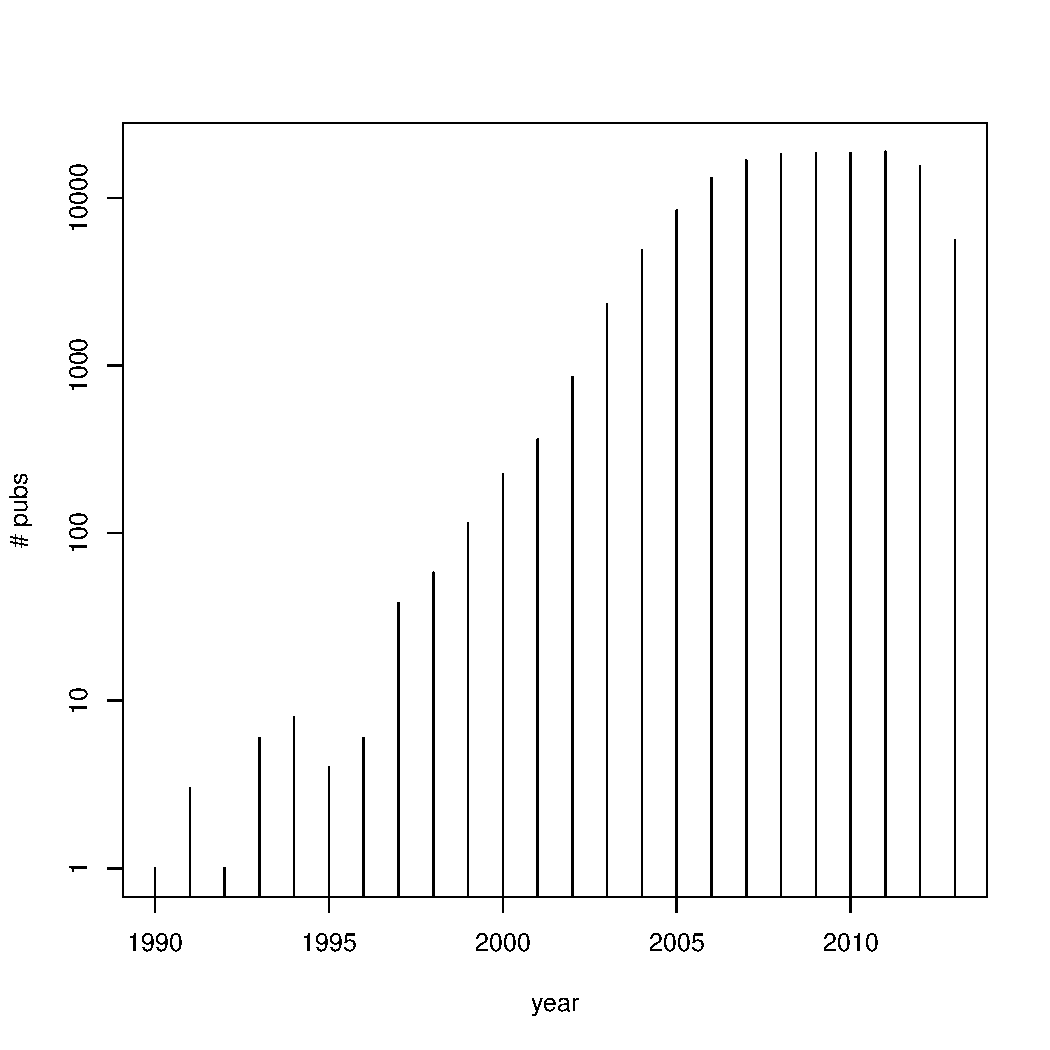
\includegraphics[width=1.0\columnwidth]{images/21_pubs_year_distribution.pdf}
  \caption{Publications by Year}\label{F:pubs-year-distribution}
\end{figure}

\begin{figure}[htb]
  \centering
    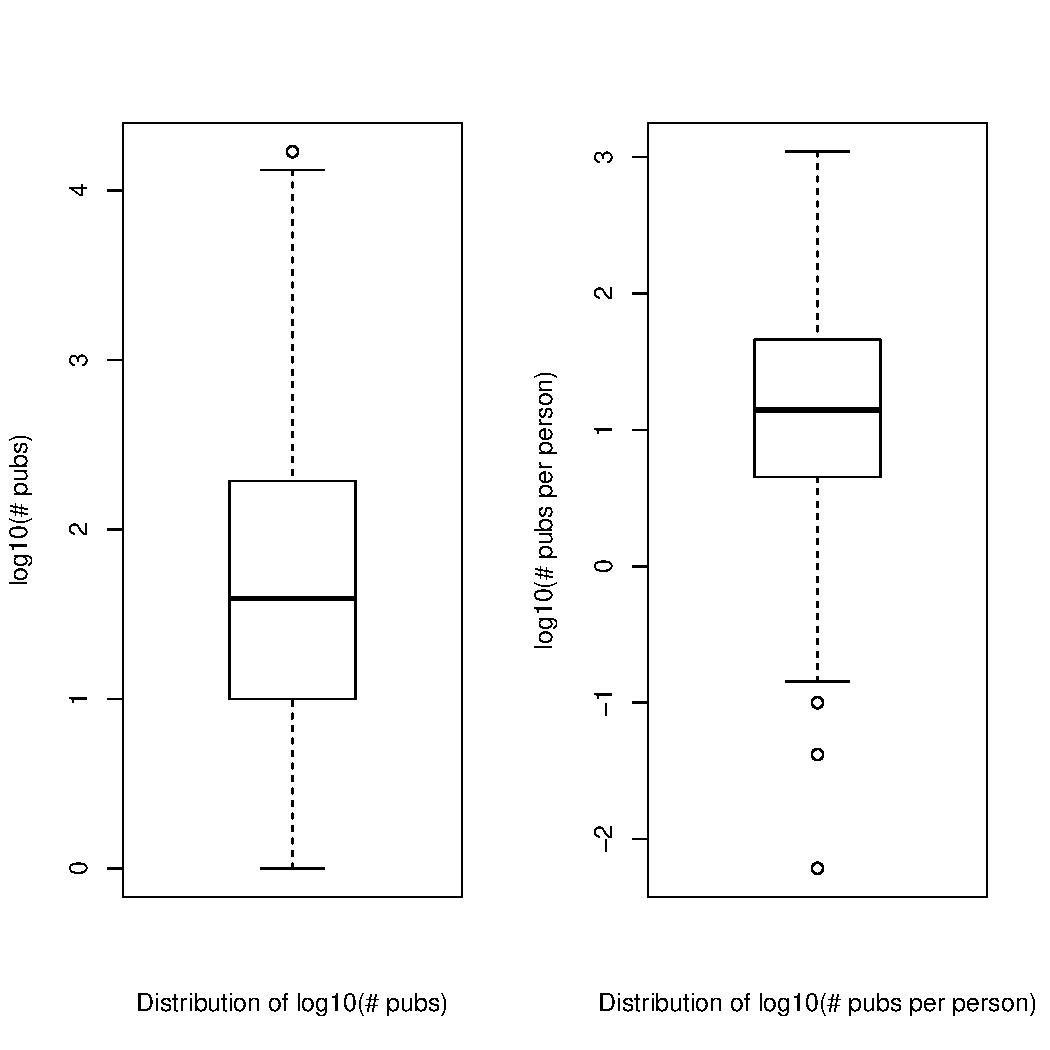
\includegraphics[width=1.0\columnwidth]{images/01_dist_npubs_proj.pdf}
  \caption{Distribution of number of publications}\label{F:dist-npubs-proj}
\end{figure}

We started the project by following the automated approach to obtain publication data. Publication citation data are available via subscribed resources such as ISI Web of Science \cite{www-isiwos} or open access such as Google Scholar \cite{www-googlescholar}, Microsoft Academic Search \cite{www-msas}, and Mendeley \cite{www-mendeley}, however they usually don't provide unlimited access.

Another approach which is probably more ideal is to get publication data from users. The user curated data tend to be more accurate comparing to automated mining, besides, there is another benefit that it gives extra information regarding a publication's association with the system, e.g., to which project it belongs. FutureGrid leveraged the drupal biblio module \cite{www-drupal-bib} with some customized design to support easy publication report and mass import via users or a staff member, and associated the publications with the related projects \cite{www-fgbiblio}. XSEDE now also provides a similar functionality via the portal \cite{www-xdportalpub}. nanoHUB citation analysis \cite{www-nanohubcite} as we have mentioned is also based on publication data submitted by users via a web form.

The framework itself supports pluggable data sources via mining databases and/or accessing 3rd party service APIs. We have experimented various data sources including Microsoft Academic Search, Google Scholar including user profile, and mining NSF award search data that are available upon request from NSF. The obtained data are then stored into the Mashup database which provides a common interface to other components in the system as well as collaborating systems like XDMOD.

In this study we focus only on two data sources - the user submitted data via XSEDE, and the NSF award search data for automated mining. The former source has user curated data with project affiliation information, thus it could give a measure on `direct' impact of XSEDE. However as it requires users' input, the former source currently has very limited data entries. The automated way obtains publication data for XSEDE users, which are not essentially direct output of using XSEDE resources, thus provides a measure on general or `indirect' impact of XSEDE. As a XSEDE user is affiliated with accounts/projects, and the projects are part of one or more FOS, we tag one publication as being related to the projects and FOSes based on these links. This is not most ideal but it provides a means to analyze the `indirect' impact on other levels in addition to users.

Based on the stated process, we were able to obtain over 142 thousand publication entries for over 20 thousand XSEDE users as of Jan 2014. Figure \ref{F:pubs-year-distribution} shows the yearly distribution of the publications. Figure \ref{F:dist-npubs-proj} shows distribution of number of publications by project (on the left) and by per user for each project.

\subsection{Citation Data Retrieval}

While for publication data user curated data might be more ideal, for citation data we have to go to the automated way for better accuracy and common grounds to compare. Google Scholar and ISI Web of Science provide such data, with some noticeable limitations. E.g., Google Scholar does not provide an API, nor it allows unlimited access within a bounded time period from one request source. ISI data does not impose a rate limiting while you have subscribed access, however it does not provide easy access API either. So one has to submit query via the web UI and then parse the data from the tabulated results list.

We have explored both approaches for a subset of the publication data, and did a comparison of the results. While similar comparison has been attempted \cite{yang2006citation} in a very small sample size - 2 people and about 100 publications, our study has included 33861 publications and 1462 users.

\begin{figure}[htb]
  \centering
    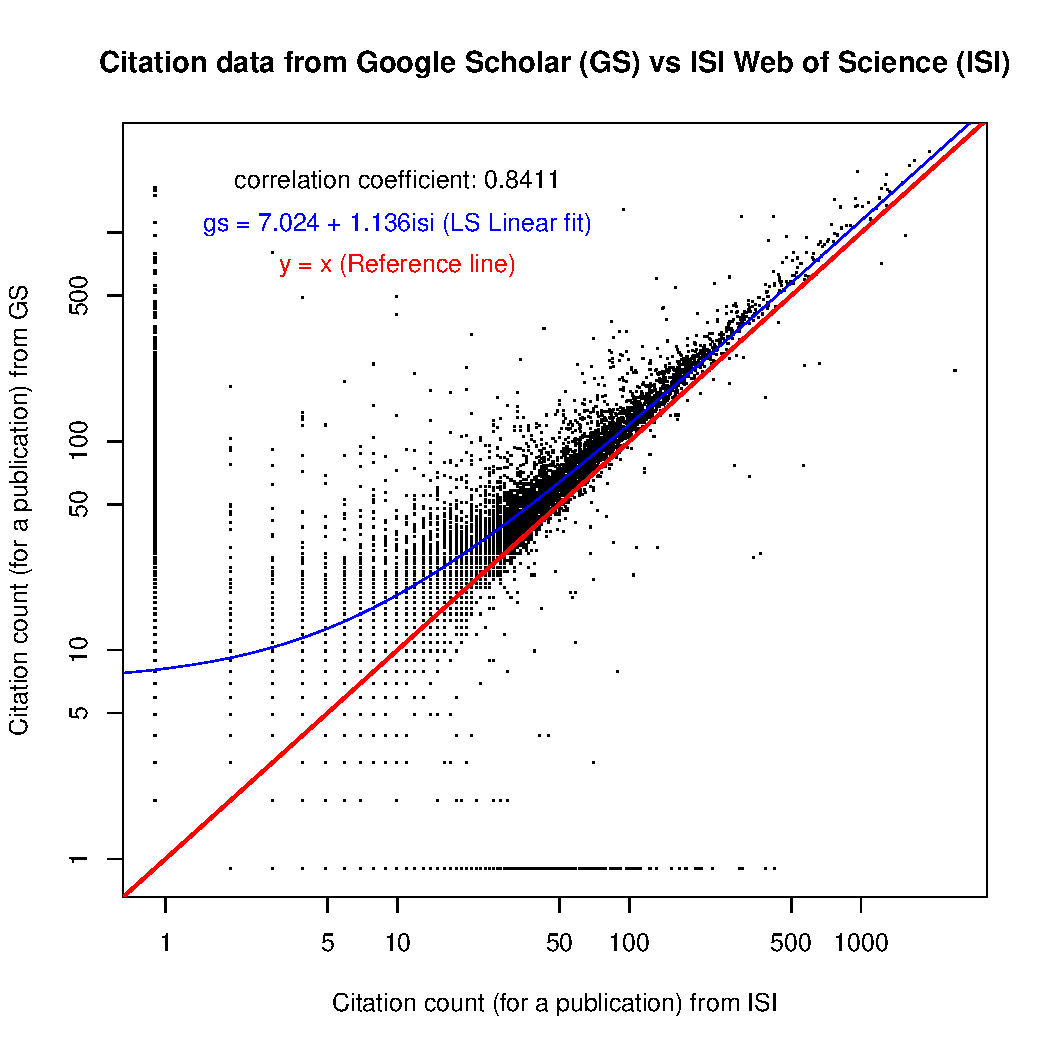
\includegraphics[width=1.0\columnwidth]{images/11_gs_vs_isi_cites.pdf}
  \caption{Citations (GS vs ISI)}\label{F:gs-vs-isi-cites}
\end{figure}

\begin{figure}[htb]
  \centering
    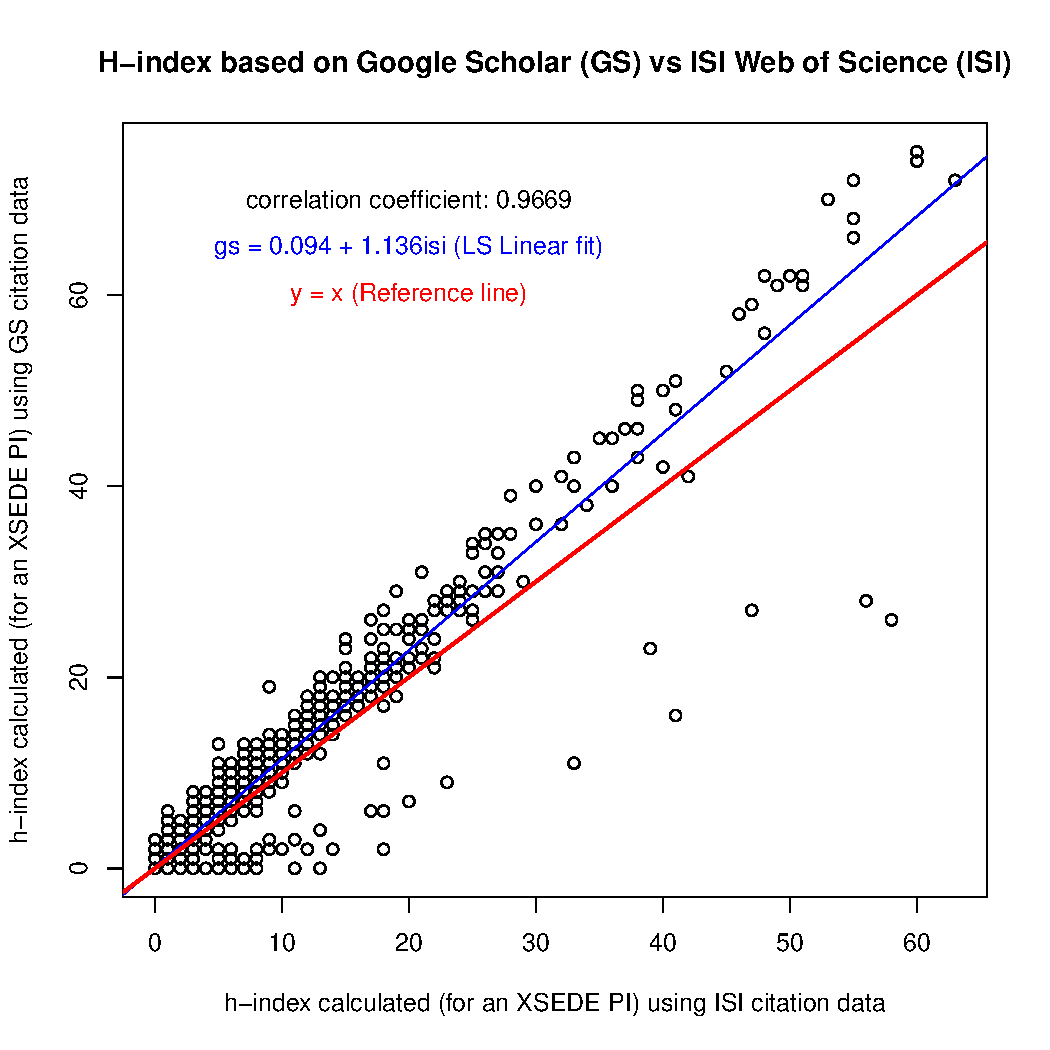
\includegraphics[width=1.0\columnwidth]{images/11_gs_vs_isi_hindex.pdf}
  \caption{H-index (GS vs ISI)}\label{F:gs-vs-isi-hindex}
\end{figure}

Figure \ref{F:gs-vs-isi-cites} shows the citation data from Google Scholar vs ISI Web of Science. Out of the 33861 data points, 20793 of them (61.4\%) have larger value in GS, 10315 (30.5\%) are the same, while 2753 (8.1\%) have larger value in ISI. 5287 (15.6\%) publications have zero citation found in ISI but non-zero in GS, 1253 (3.7\%) pubs have zero citaion in GS but non-zero in ISI. In general Google Scholar tends to have higher citation number.

Figure \ref{F:gs-vs-isi-hindex} shows that H-index obtained from Google Scholar data vs ISI data. Out of the 1462 data points, 663 of them (45.3\%) have larger value in GS, 677 (46.3\%) are the same, while 122 (8.3\%) have larger value in ISI.
52 (3.6\%) PIs have zero H-index computed from ISI data but non-zero from GS, 39 (2.7\%) for the reverse side. In general h-index calculated from Google Scholar data tends to be a bit higher.

In either case a high positive correlation is observed. The Pearson correlation coefficient are 0.84 and 0.97 respectively. The very strong correlation of the h-index values are mostly due to the fact that one of the two factors determining the h-index, the number of publications, stay the same for a perticular user.

Based on the study, while we don't have complete citation data from Google Scholar due to access restriction, we were able to use the ISI citation data to get very similar measures for most of the data especially for the h-index metric. Thus the following analyses are using the ISI citation data to further derive other metrics.

\section{Results and Analyses}

The previous section showed the data we have obtained. In this section we will discuss the metrics derived from those data to evaluate the impact. We will also do analyses when correlating the metrics to the XSEDE correlation data to show how the impact is reflected on different levels, e.g. by FOS.

\subsection{Direct impact of XSEDE}

\begin{figure}[htb]
  \centering
    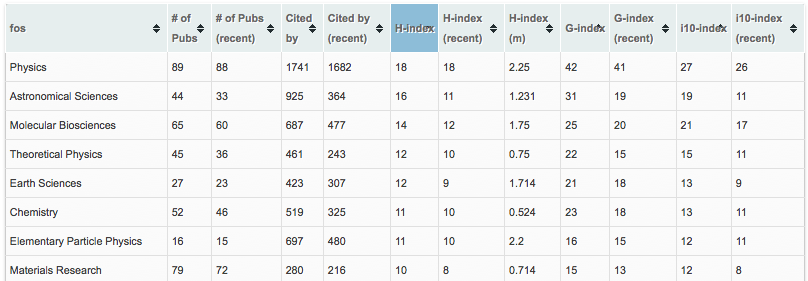
\includegraphics[width=1.0\columnwidth]{images/XDPUBS_Metrics_FOS.png}
  \caption{Metrics in FOS level}\label{F:xdpubs-metrics-fos}
\end{figure}

By using the user submitted publication entries only, which are tagged as `direct' output of XSEDE projects, we were able to show the `direct' impact of XSEDE. E.g., as of Jan 27, 2014, the 837 publications involved 882 XSEDE users as authors, and 220 organizations, 331 XSEDE projects, and received 11,258 citations to date. We have calculated the various metrics on the level of user, organization, projects, and FOS involved. Figure \ref{F:xdpubs-metrics-fos} shows the top most impact FOSes judging by h-index values.

\subsection{Project metrics vs SUs allocation}

\begin{figure}[htb]
  \centering
    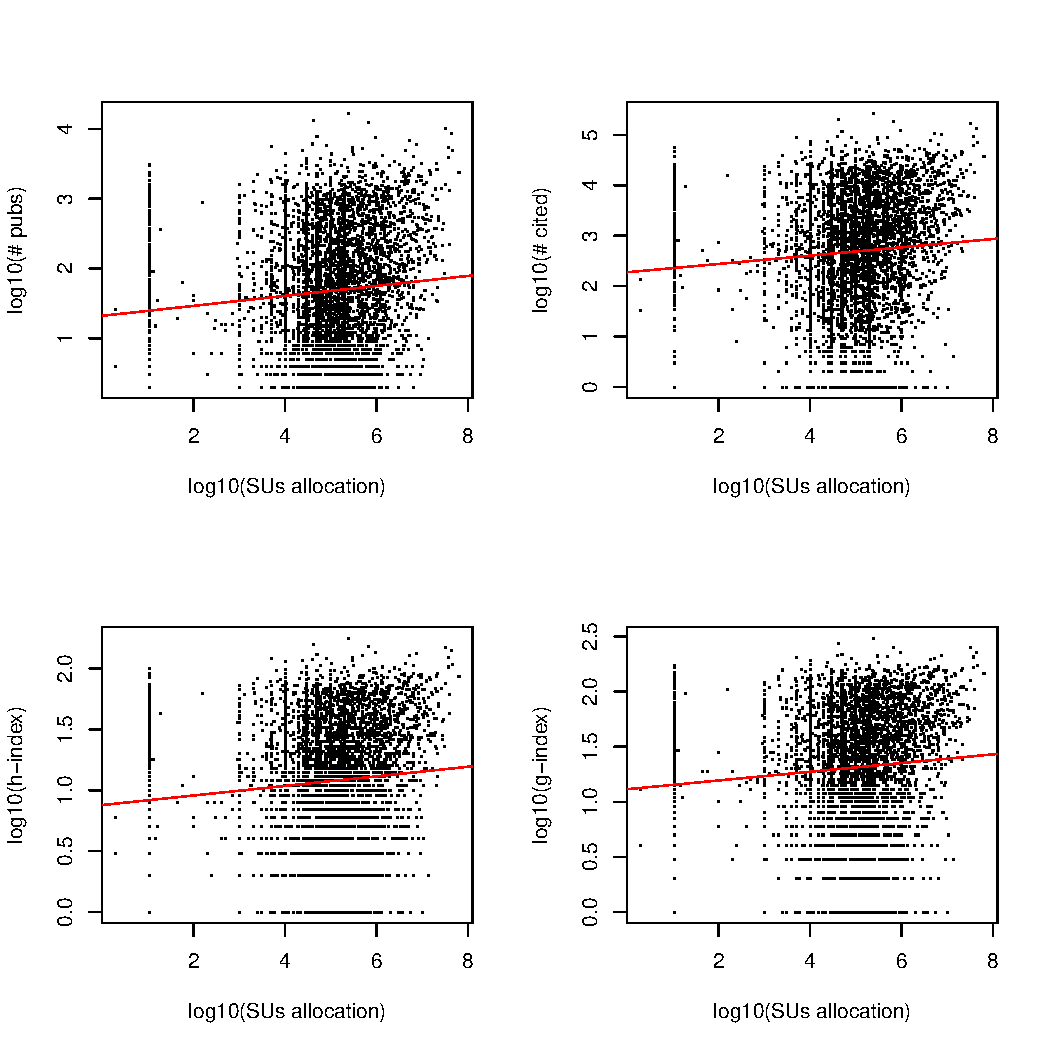
\includegraphics[width=1.0\columnwidth]{images/02_metrics_vs_alloc_proj.pdf}
  \caption{Metrics vs SUs for all projects}\label{F:metrics-vs-alloc-proj}
\end{figure}

\begin{figure}[htb]
  \centering
    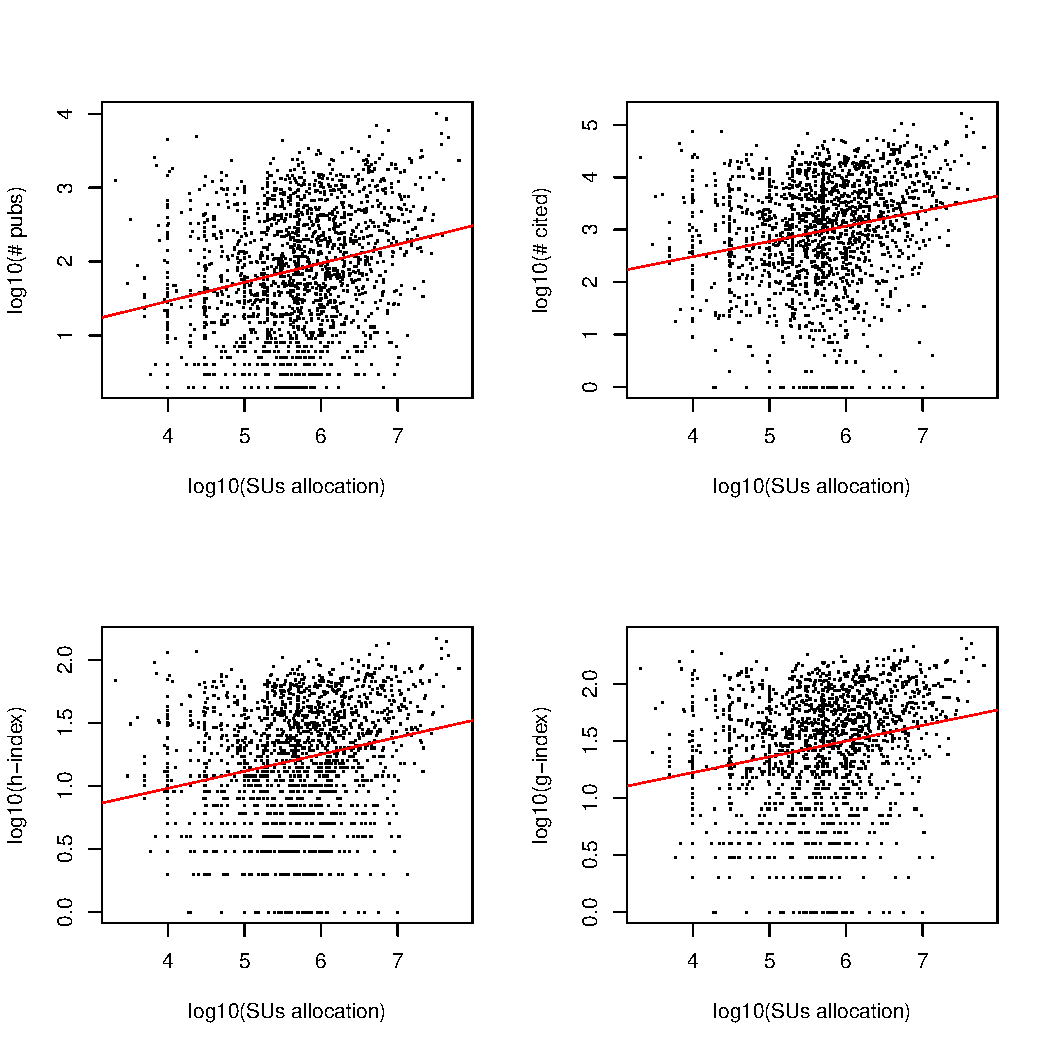
\includegraphics[width=1.0\columnwidth]{images/02_metrics_vs_alloc_research_proj.pdf}
  \caption{Metrics vs SUs for research projects}\label{F:metrics-vs-alloc-research-proj}
\end{figure}

%\begin{figure}[htb]
%  \centering
%    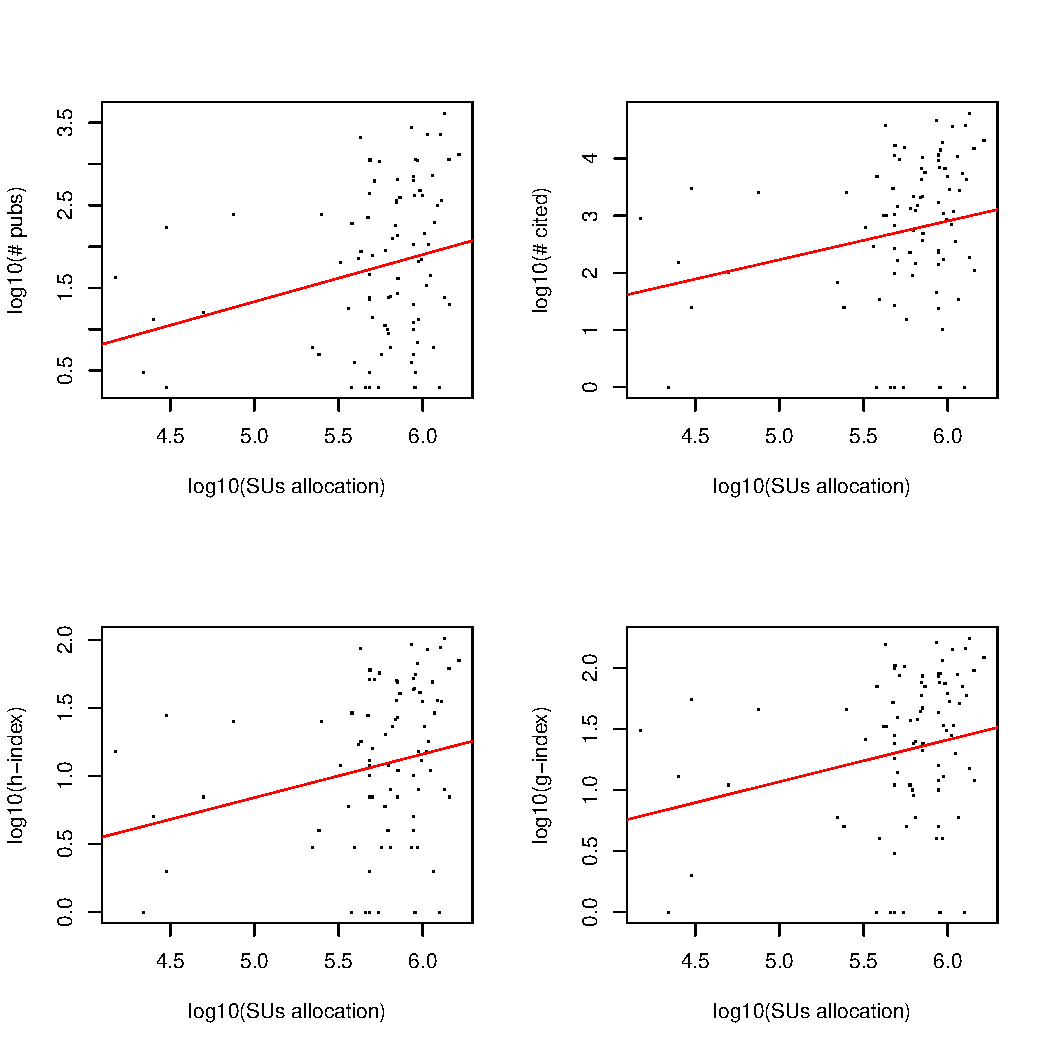
\includegraphics[width=1.0\columnwidth]{images/02_metrics_vs_alloc_campus_proj.pdf}
%  \caption{Metrics vs SUs for campus champion projects}\label{F:metrics-vs-alloc-campus-proj}
%\end{figure}

%\begin{figure}[htb]
%  \centering
%    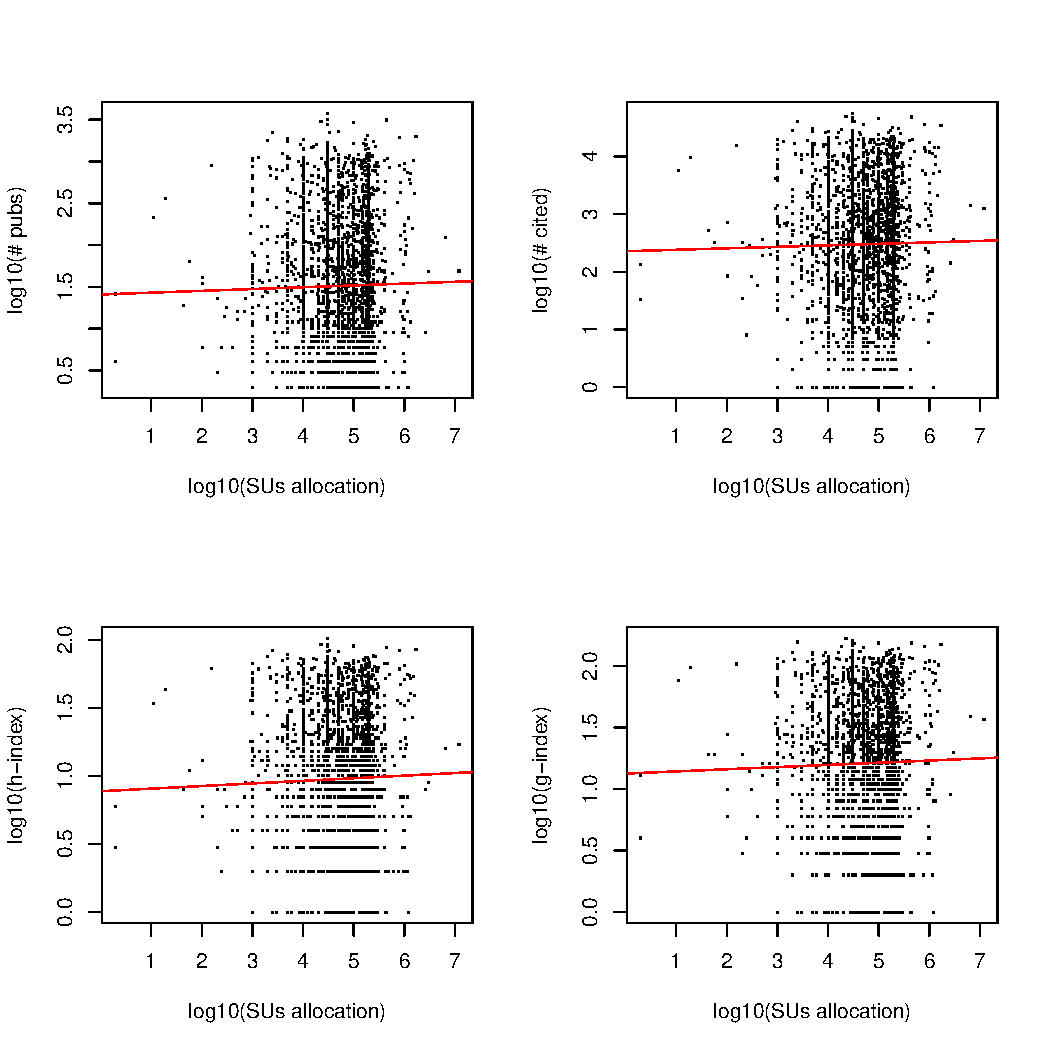
\includegraphics[width=1.0\columnwidth]{images/02_metrics_vs_alloc_startup_proj.pdf}
%  \caption{Metrics vs SUs for startup projects}\label{F:metrics-vs-alloc-startup-proj}
%\end{figure}

\begin{table}[htb]
  \centering
    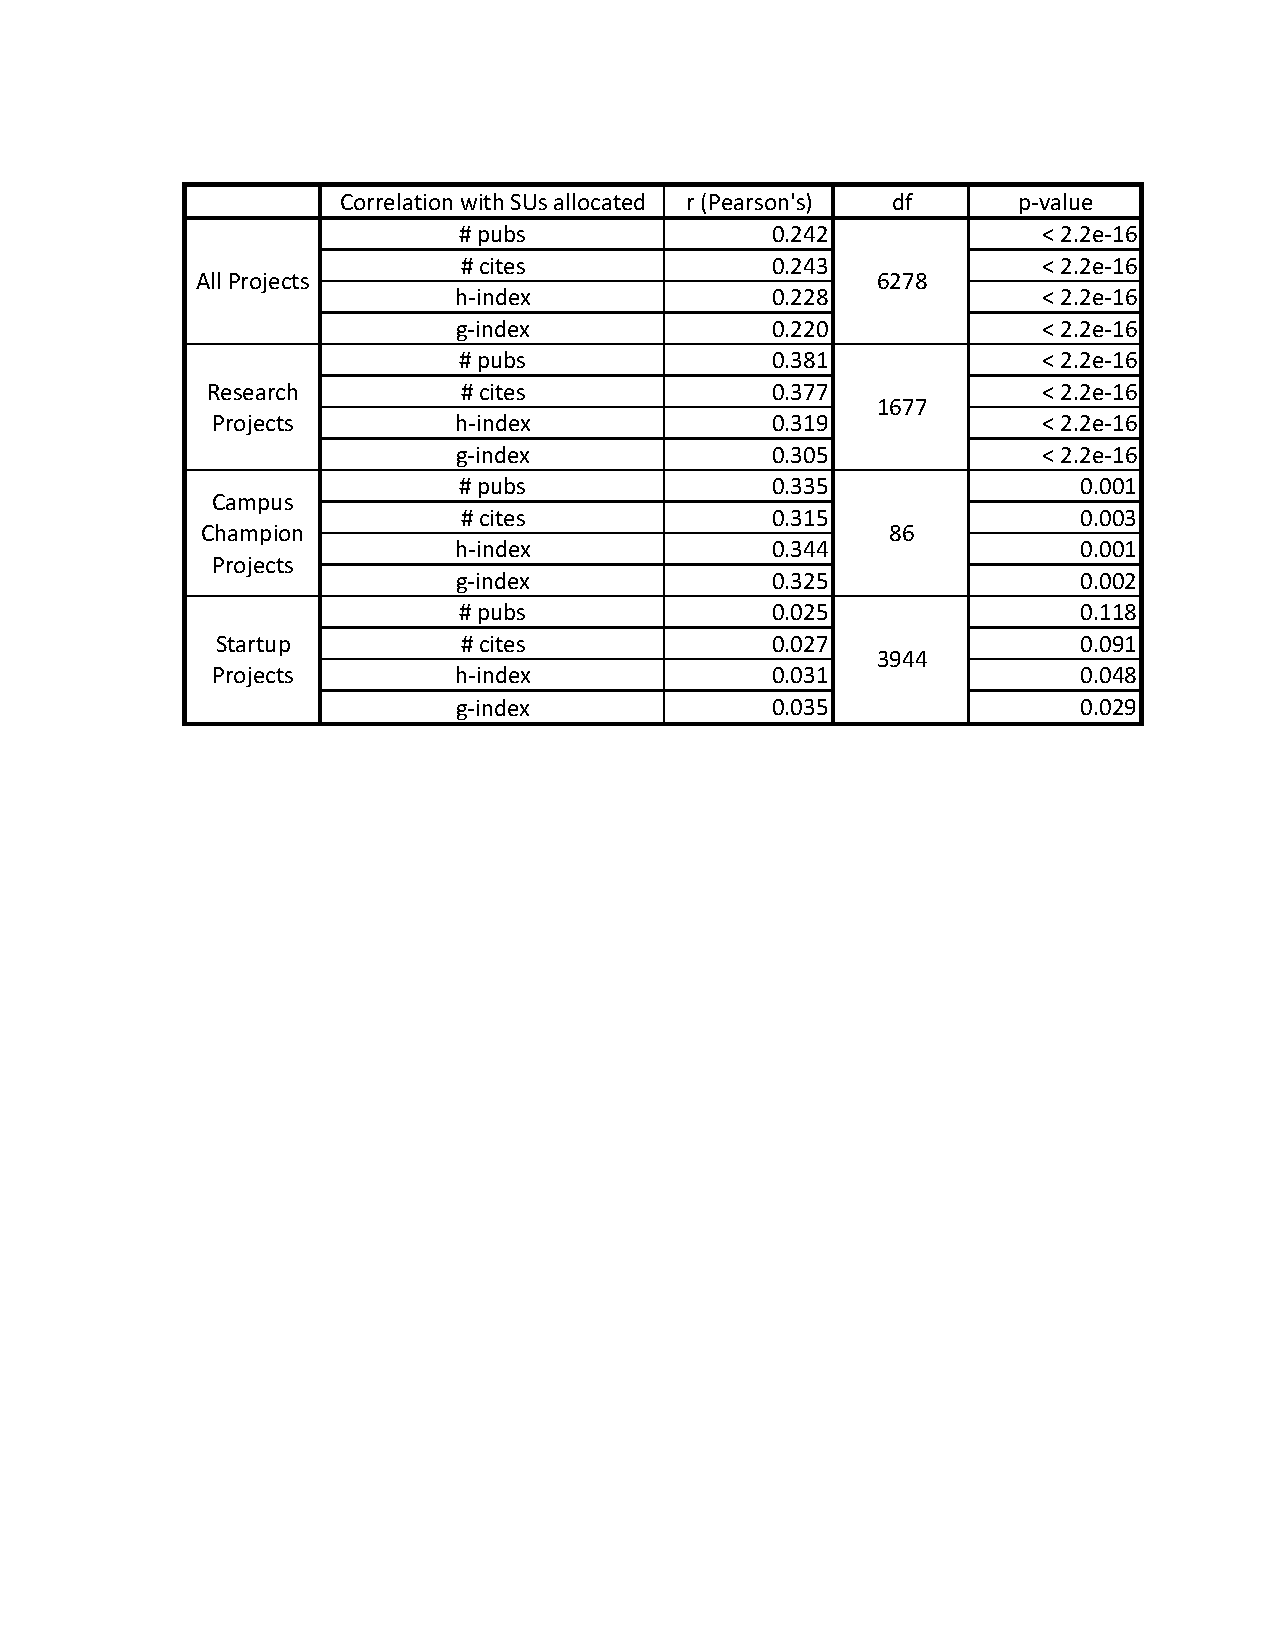
\includegraphics[width=1.0\columnwidth]{images/metrics_alloc_r.pdf}
  \caption{Correlation between SUs allocated vs the metrics for each project}\label{F:metrics-alloc-r}
\end{table}

Figure \ref{F:metrics-vs-alloc-proj} showed the correlation analysis of impact metrics and XD resource allocation on individual project level based on all projects data. While previous work showed stronger correlation between the citation and SUs \cite{bollen2011and} in much smaller sample size from one certain resource allocation meeting, we observed weaker correlation, if any. When categorizing the projects based on the types, e.g., research, startup, campus champion, etc., it shows a stronger, although still not strong, correlation in each category other than for the startup projects. Figure \ref{F:metrics-vs-alloc-research-proj} showed the analysis for research projects only. Table \ref{F:metrics-alloc-r} listed the correlation coefficient values as well as the p-values showing the significance of the test. Please note in Figure \ref{F:metrics-vs-alloc-proj} and \ref{F:metrics-vs-alloc-research-proj} we included a regression lines showing the upper trends of the correlation, i.e., higher SUs allocation correlating to higher impact metrics, but not suggesting the linear relationship. This correlation analysis does not show the cause effect either, as in this case it's very likely that the causal are reciprocal.

\subsection{Metrics vs SUs allocation on FOS level}

\begin{figure}[htb]
  \centering
    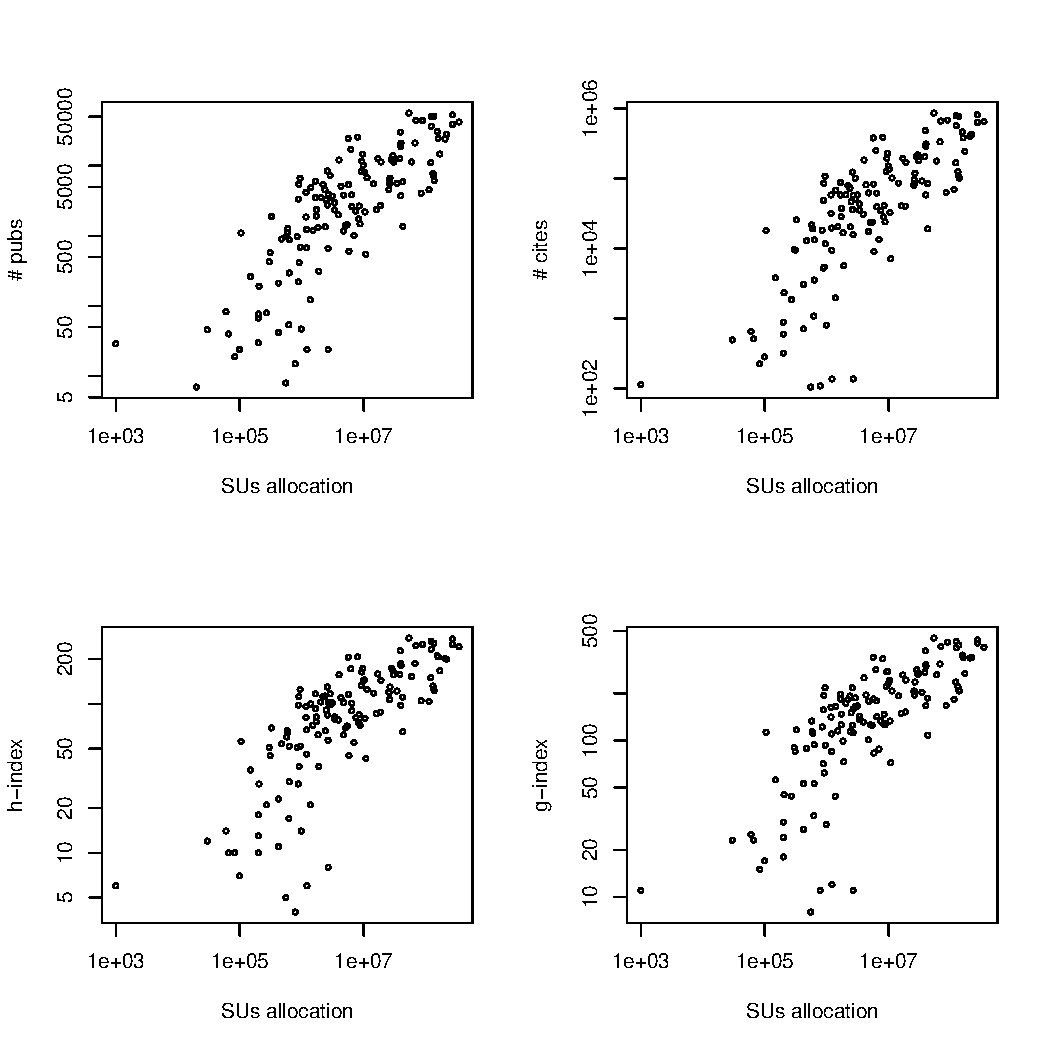
\includegraphics[width=1.0\columnwidth]{images/03_metrics_vs_alloc_fos.pdf}
  \caption{Metrics vs SUs for FOSes}\label{F:metrics-vs-alloc-fos}
\end{figure}
While on individual project level we don't observe strong correlations between impact metrics vs the resource allocations, Figure \ref {F:metrics-vs-alloc-fos} shows stronger positive correlation on FOS level. The Pearson correlation coefficient are 0.704, 0.712, 0.651, 0.648 respectively. With a degree of freedom at 132 and p-values less than 2.2e-16 from the test, it shows very high statistical significance. 

%\begin{figure}[htb]
%  \centering
%    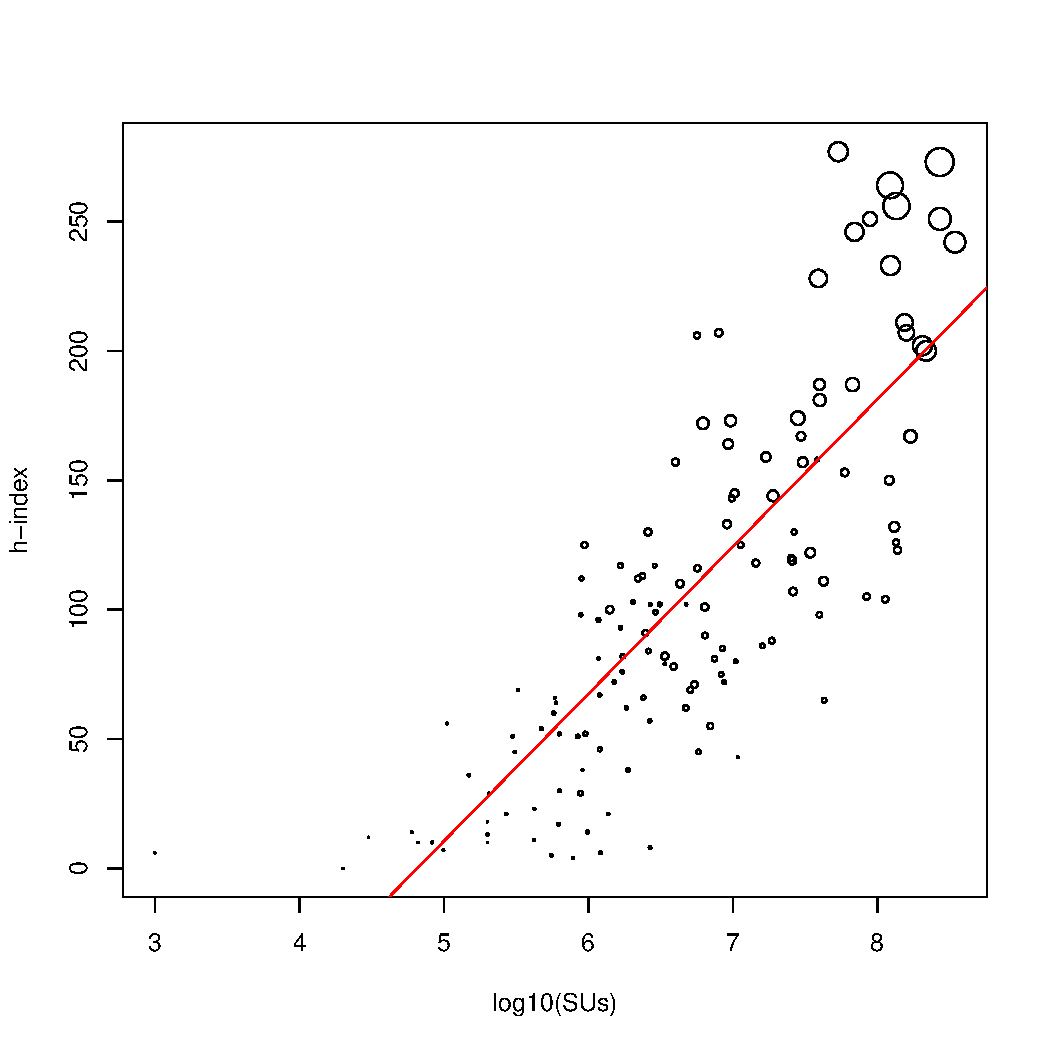
\includegraphics[width=1.0\columnwidth]{images/04_hindex_vs_alloc_fos_sized.pdf}
%  \caption{h-index (sized by size of FOS) vs allocation}\label{F:hindex-vs-alloc-fos-sized}
%\end{figure}

\begin{figure}[htb]
  \centering
    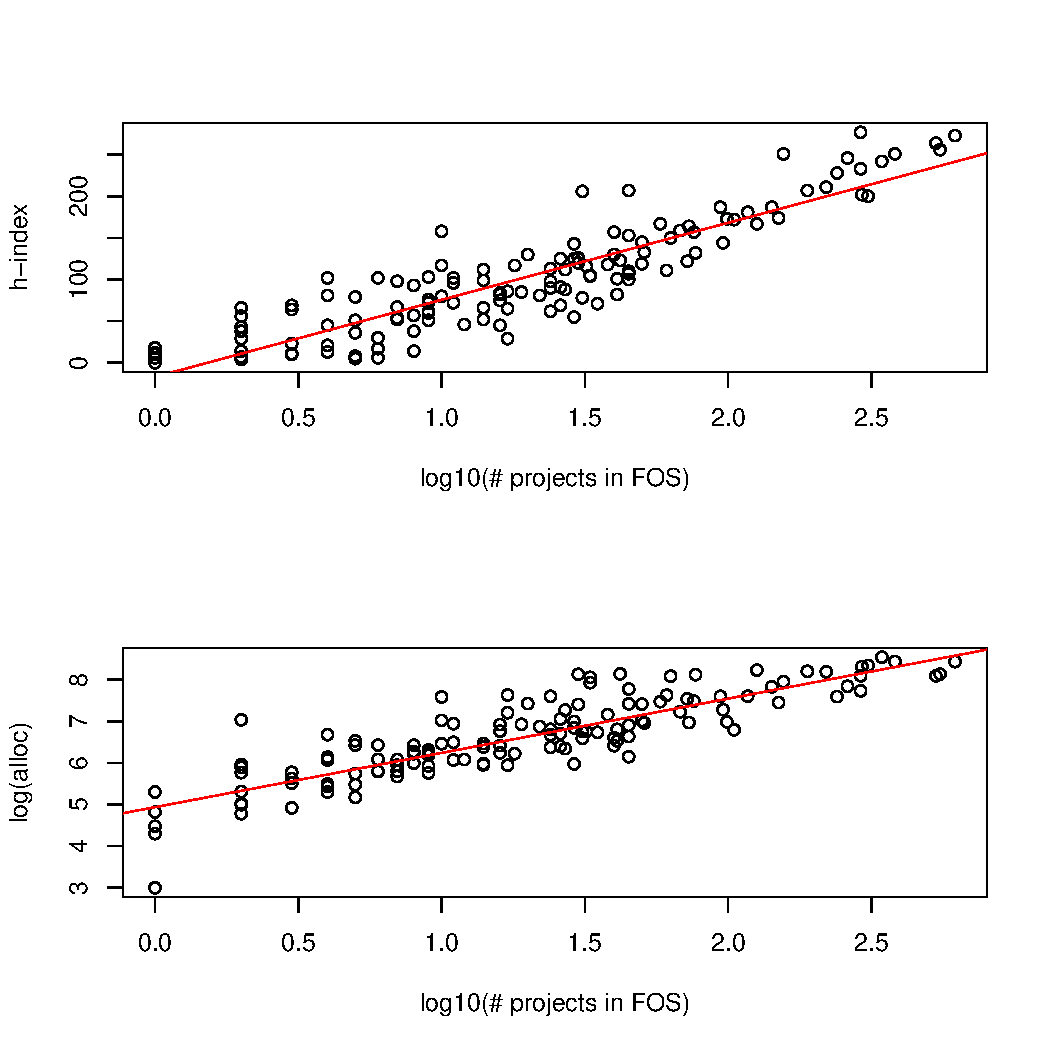
\includegraphics[width=1.0\columnwidth]{images/05_hindexalloc_vs_nprojects_fos_trended.pdf}
  \caption{Effects of sizes of FOSes}\label{F:hindexalloc-vs-nprojects-fos-trended}
\end{figure}

However as Figure \ref{F:hindexalloc-vs-nprojects-fos-trended} suggests, the stronger correlations are mostly caused by the effect of different size of the FOSes, judging by number of projects each FOS has. But this does not diminish the purpose of the analysis showing how XSEDE could impact science from different disciplines, e.g., by approving more projects and granting more allocations for certain FOSes.

\begin{figure}[htb]
  \centering
    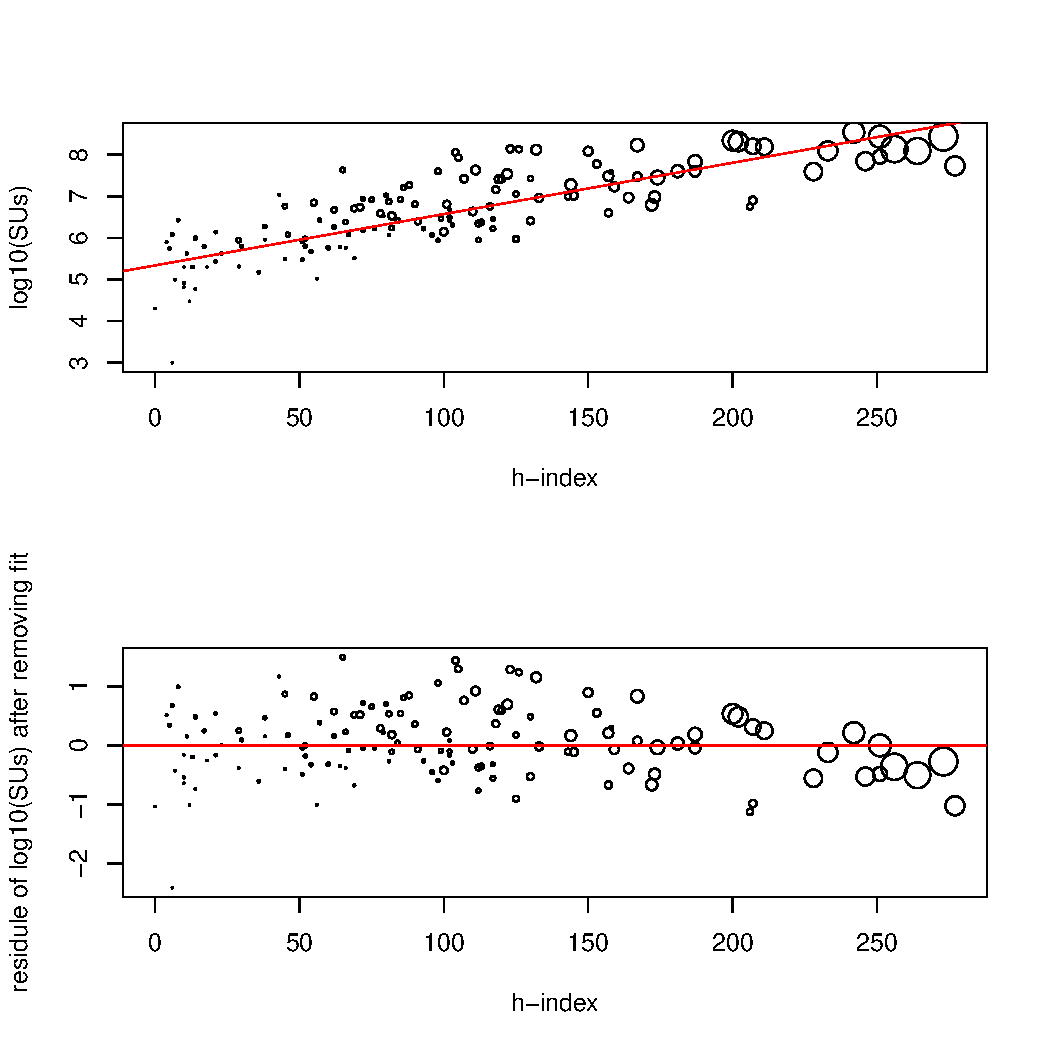
\includegraphics[width=1.0\columnwidth]{images/05_alloc_vs_hindex_fos_sized_2in1.pdf}
  \caption{SUs vs h-index for each FOS with trend (above) and residual analysis (bottom)}\label{F:alloc-vs-hindex-fos-sized}
\end{figure}

%\begin{figure}[htb]
%  \centering
%    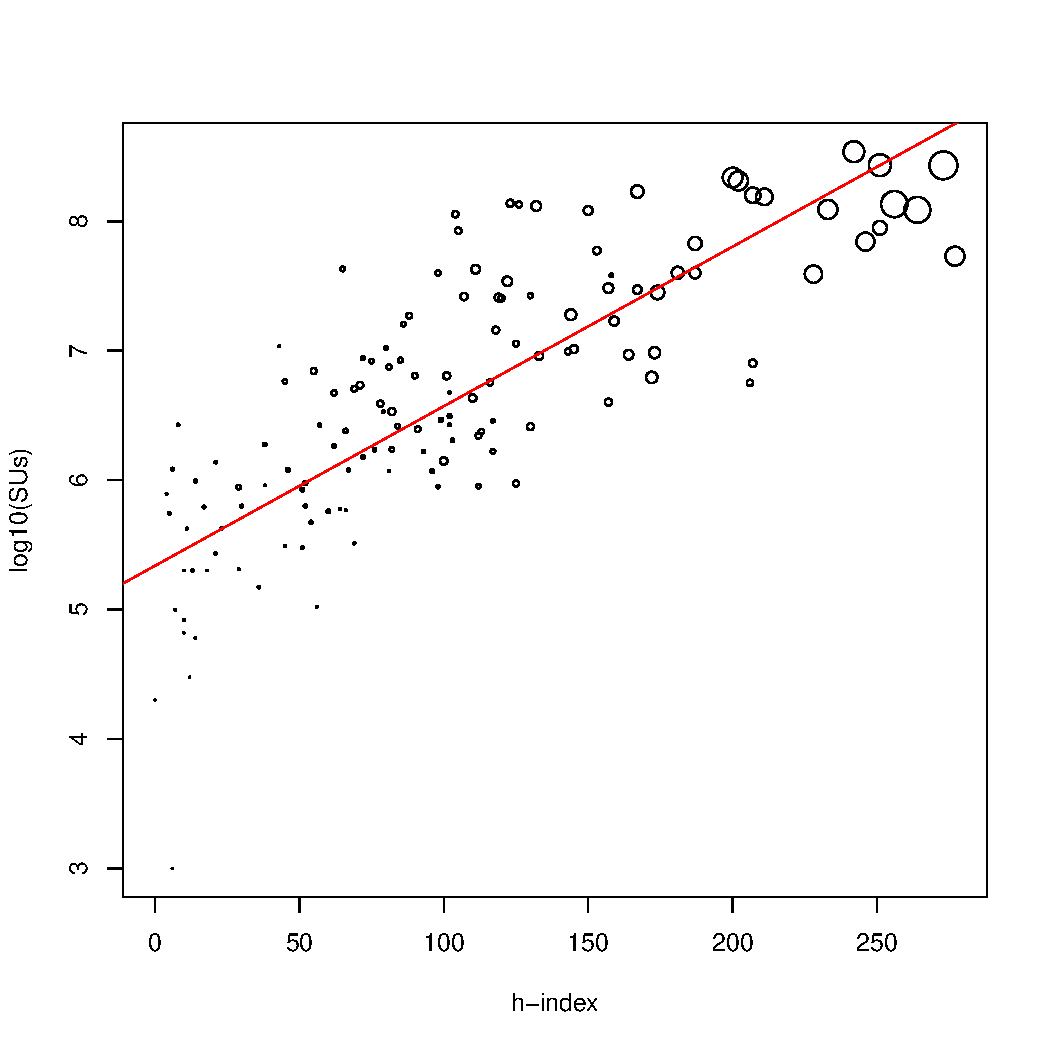
\includegraphics[width=1.0\columnwidth]{images/05_alloc_vs_hindex_fos_sized_trended.pdf}
%  \caption{SUs vs h-index for each FOS with trend}\label{F:alloc-vs-hindex-fos-sized-trended}
%\end{figure}

%\begin{figure}[htb]
%  \centering
%    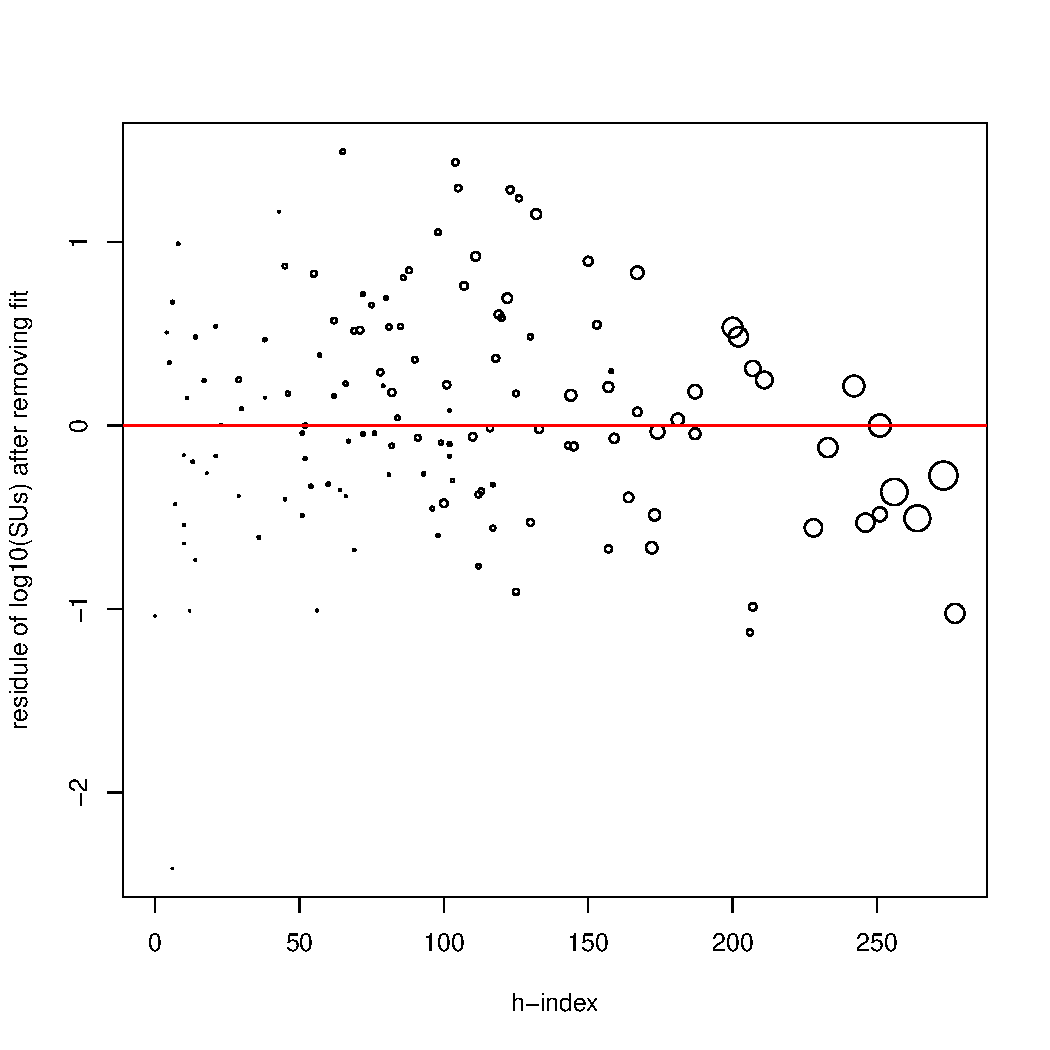
\includegraphics[width=1.0\columnwidth]{images/05_alloc_vs_hindex_fos_sized_residual.pdf}
%  \caption{Residual analysis of SUs vs h-index}\label{F:alloc-vs-hindex-fos-sized-residual}
%\end{figure}

\begin{figure}[htb]
  \centering
    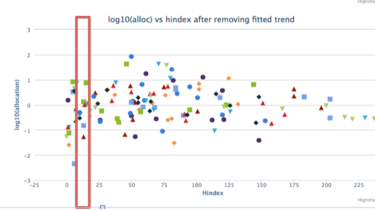
\includegraphics[width=1.0\columnwidth]{images/fig3.pdf}
  \caption{Interactive SUs vs h-index on FOS level}\label{F:fig3}
\end{figure}

Figure \ref{F:alloc-vs-hindex-fos-sized} showed the SUs received (transformed in logarithmic scale) vs the h-index produced for each FOS, while the circle size proportional to the size (number of projects) of the FOS. It also showed that after removing the fitted trend, we could see the diverging of the SUs received, from the expected SUs trend to produce the given impact judging by h-index. This could imply that certain FOSes are more efficiently to produce the given impact while some others are requiring more than expected SUs to produce the given impact. To further facilitate this analysis, we have an interactive version of the plot in our web portal as shown in Figure \ref{F:fig3}. It helps to make the following observations:

\begin{enumerate}

\item We find that several FOS with the similar h-index use fewer resources than others showing better relative output measured by the h-index. This is done by comparing FOS on a vertical slice of the h-index as seen in Figure \ref{F:fig3}

\item The trend introduces a baseline of 0. FOS above 0 use more resources than the trend, FOS bellow 0 use less resources to produce the expected impact based on a given h-index.

\item Some outliers might need more careful investigation, e.g., if more supports should be given to projects in that FOS?

\end{enumerate}

\begin{figure}[htb]
  \centering
    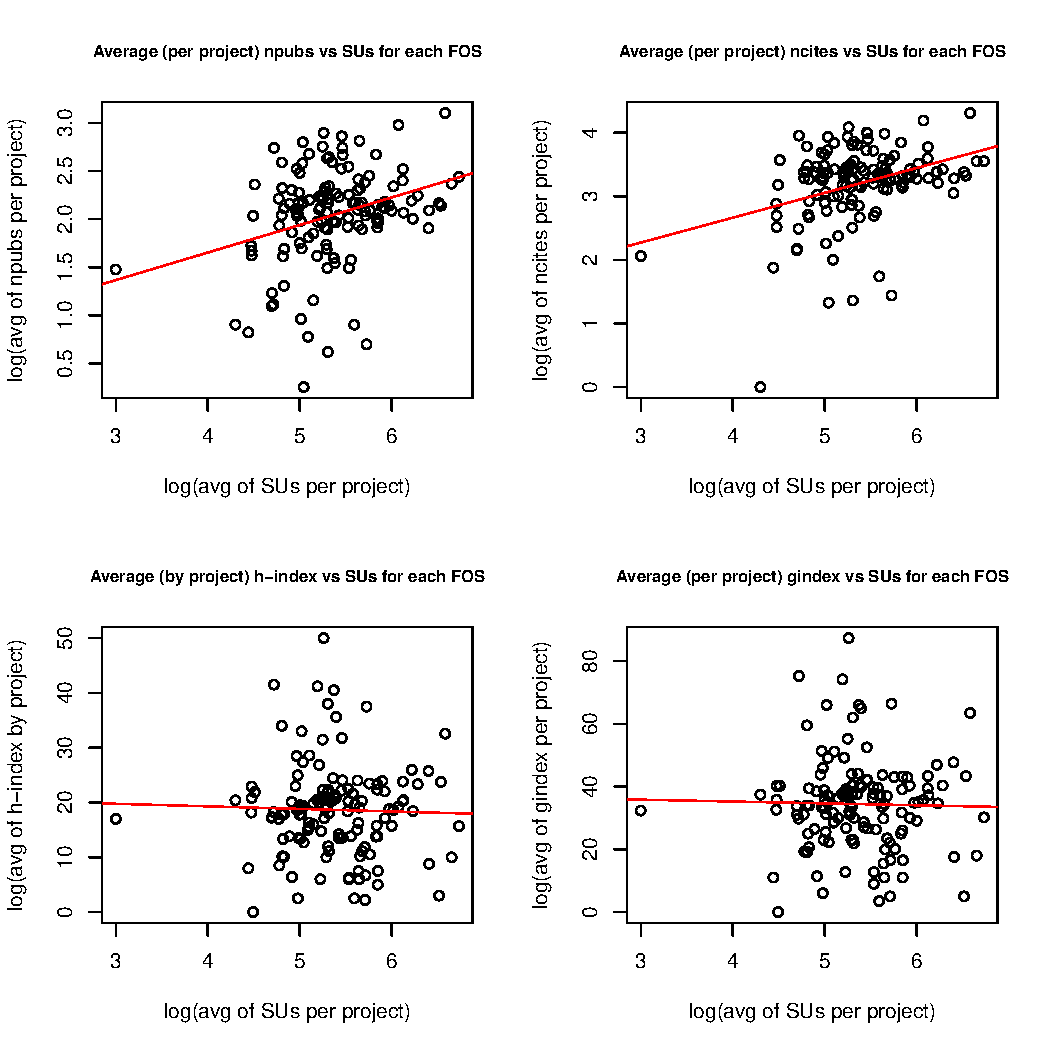
\includegraphics[width=1.0\columnwidth]{images/08_metrics_vs_alloc_avg_log_fit.pdf}
  \caption{Metrics vs SUs for FOS (avg by project)}\label{F:metrics-vs-alloc-avg-log-fit}
\end{figure}

\begin{table}[htb]
  \centering
    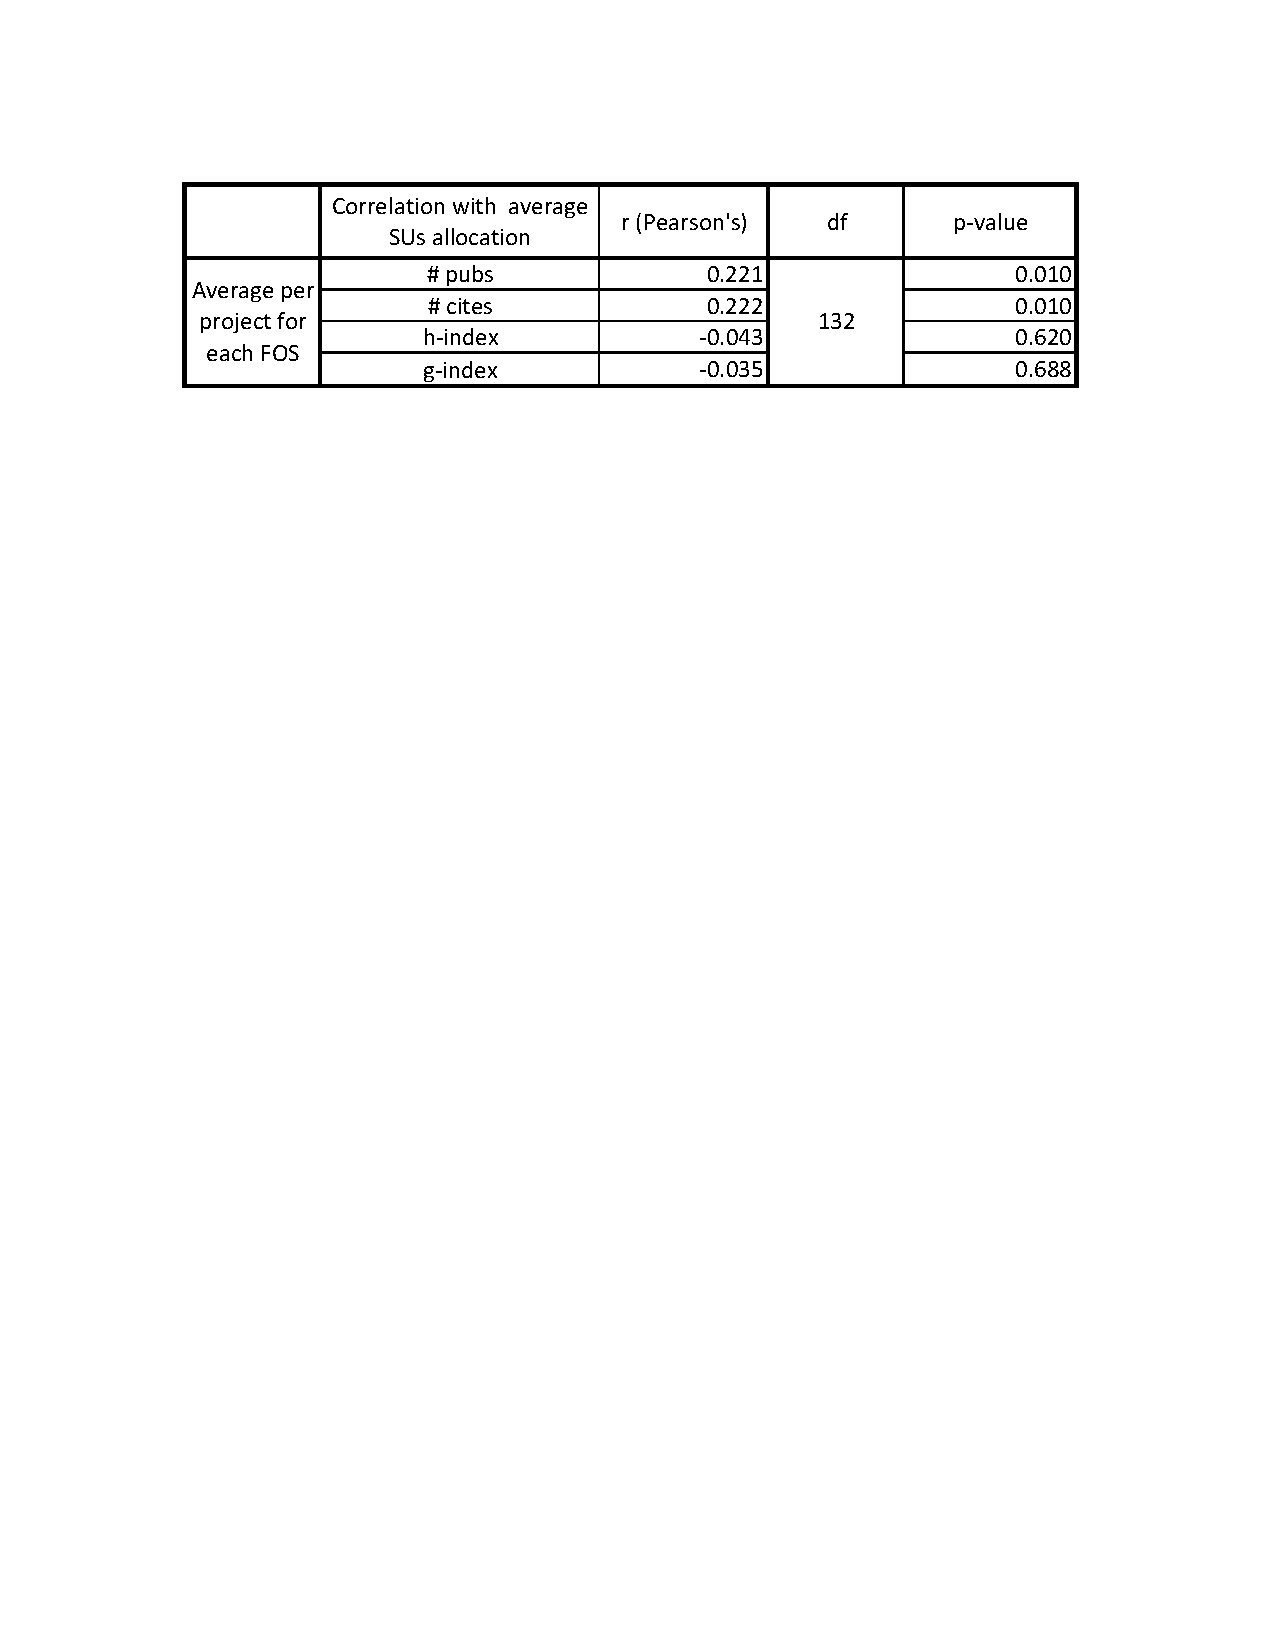
\includegraphics[width=1.0\columnwidth]{images/metrics_alloc_r_fos.pdf}
  \caption{Correlation between average SUs allocated vs the average metrics (by projects) for each FOS}\label{F:metrics-alloc-r-fos}
\end{table}

As size of FOS affects significantly the impact as well as the allocations, e.g. for h-index as in Figure \ref{F:hindexalloc-vs-nprojects-fos-trended}. We can eliminate this effect by comparing the averaging by project values within each FOS, as shown in Figure \ref{F:metrics-vs-alloc-avg-log-fit}. Table \ref{F:metrics-alloc-r-fos} has the values. It shows the weak correlation of per project based metrics vs SUs for number of publications and citations, which is actually not significantly different than the result from Table \ref{F:metrics-alloc-r}. For h-index and g-index, the test implies no correlation at all found probably due to the case that these metrics does not work well when averaging as they are not cumulative and additive values.

\begin{figure}[htb]
  \centering
    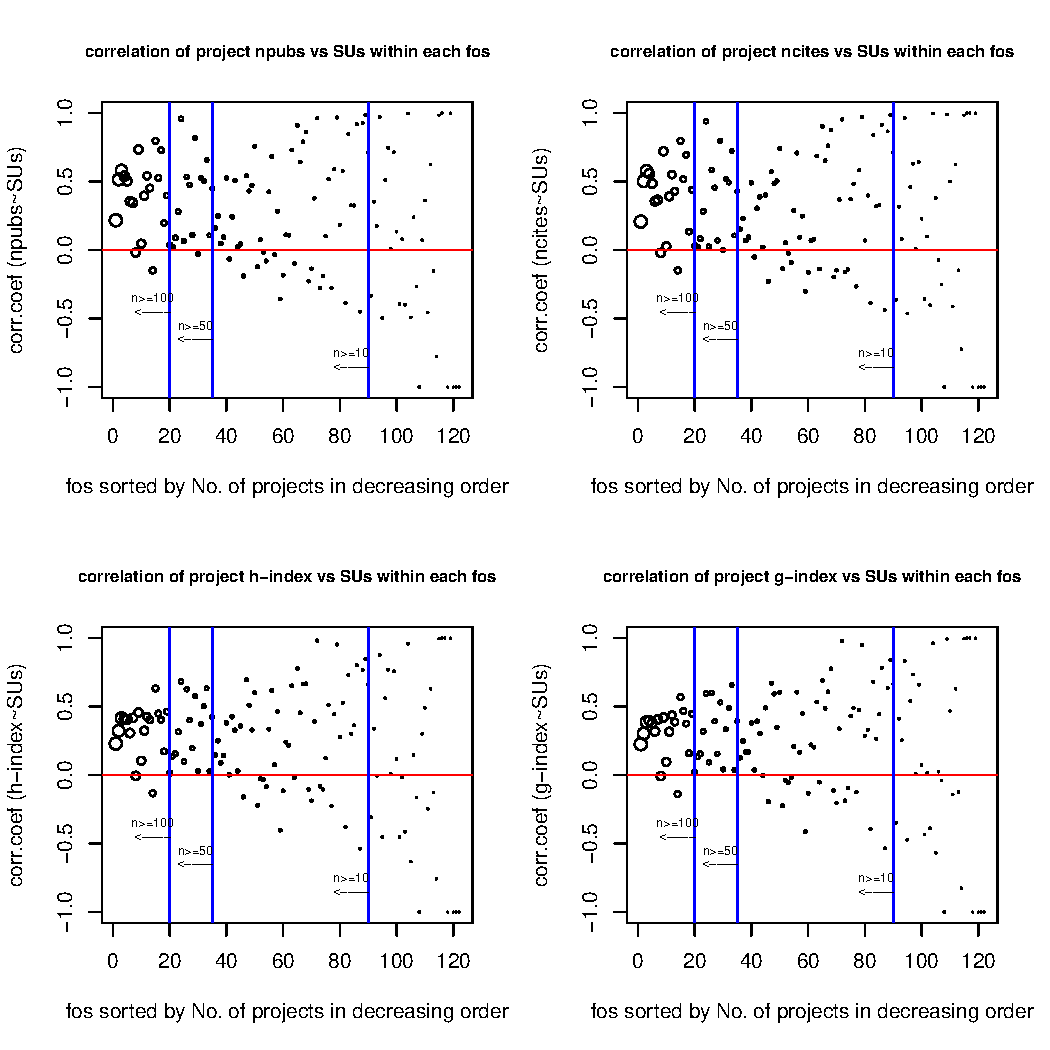
\includegraphics[width=1.0\columnwidth]{images/06_corr_metrics_vs_alloc_proj_by_fos.pdf}
  \caption{Correlations of metrics vs SUs on project level for each FOS}\label{F:corr-metrics-vs-alloc-proj-by-fos}
\end{figure}

However as shown in Figure \ref{F:corr-metrics-vs-alloc-proj-by-fos}, within each FOS, the project level metrics vs SUs correlations are typically a bit higher especially for those large size FOSes. With the increasing of size of FOS (n=10, n=50, and n=100) are denoted as vertical lines), the correlation appears positively higher and more significant. This suggests that for most FOS, impact metrics does have positive correlations with SUs allocated. Also by investigating the individual data points, we could see in which FOS this correlation appears much stronger, while for some others there are not correlation at all.

%\begin{figure}[htb]
%  \centering
%    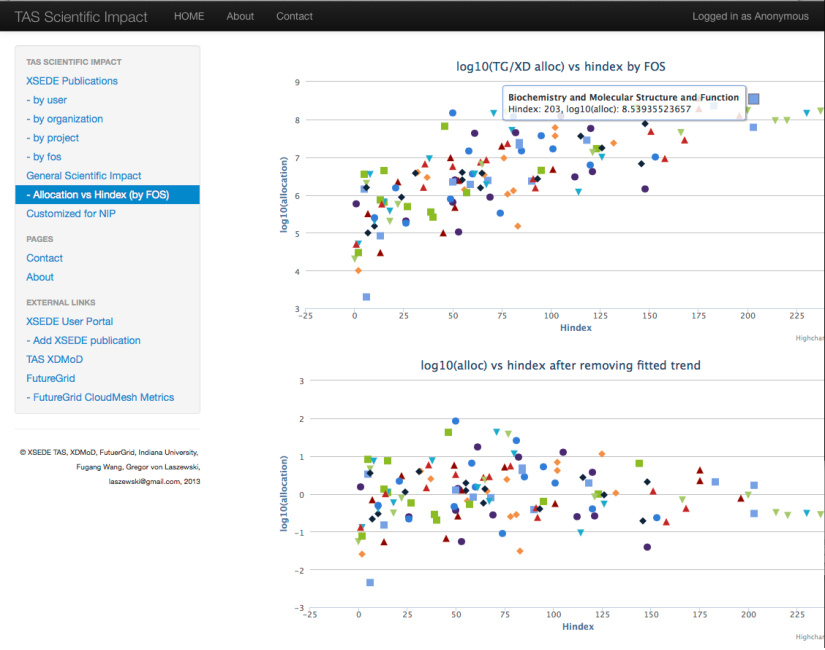
\includegraphics[width=1.0\columnwidth]{images/fig2.pdf}
%  \caption{fig2.}\label{F:fig2}
%\end{figure}

%\begin{figure}[htb]
%  \centering
%    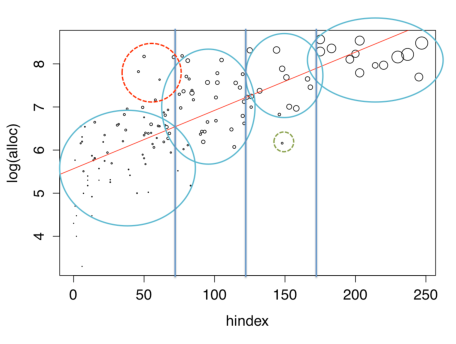
\includegraphics[width=1.0\columnwidth]{images/fig4.pdf}
%  \caption{fig4.}\label{F:fig4}
%\end{figure}

%\begin{figure*}[htb]
%  \centering
%    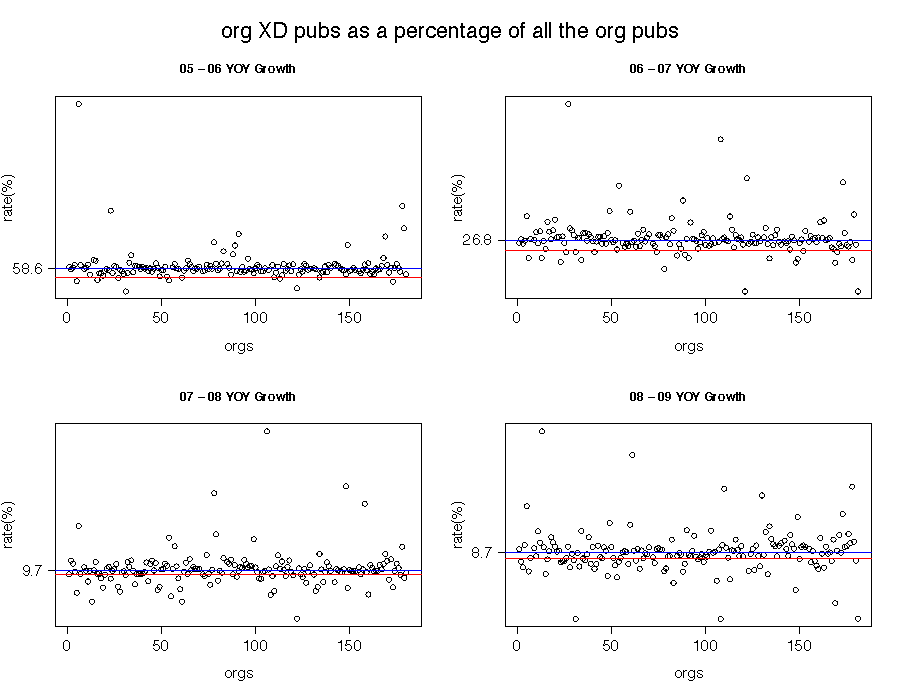
\includegraphics[width=1.0\textwidth]{images/fig5.pdf}
%  \caption{fig5.}\label{F:fig5}
%\end{figure*}

% from previous summary report

%\begin{figure}[htb]
%  \centering
%    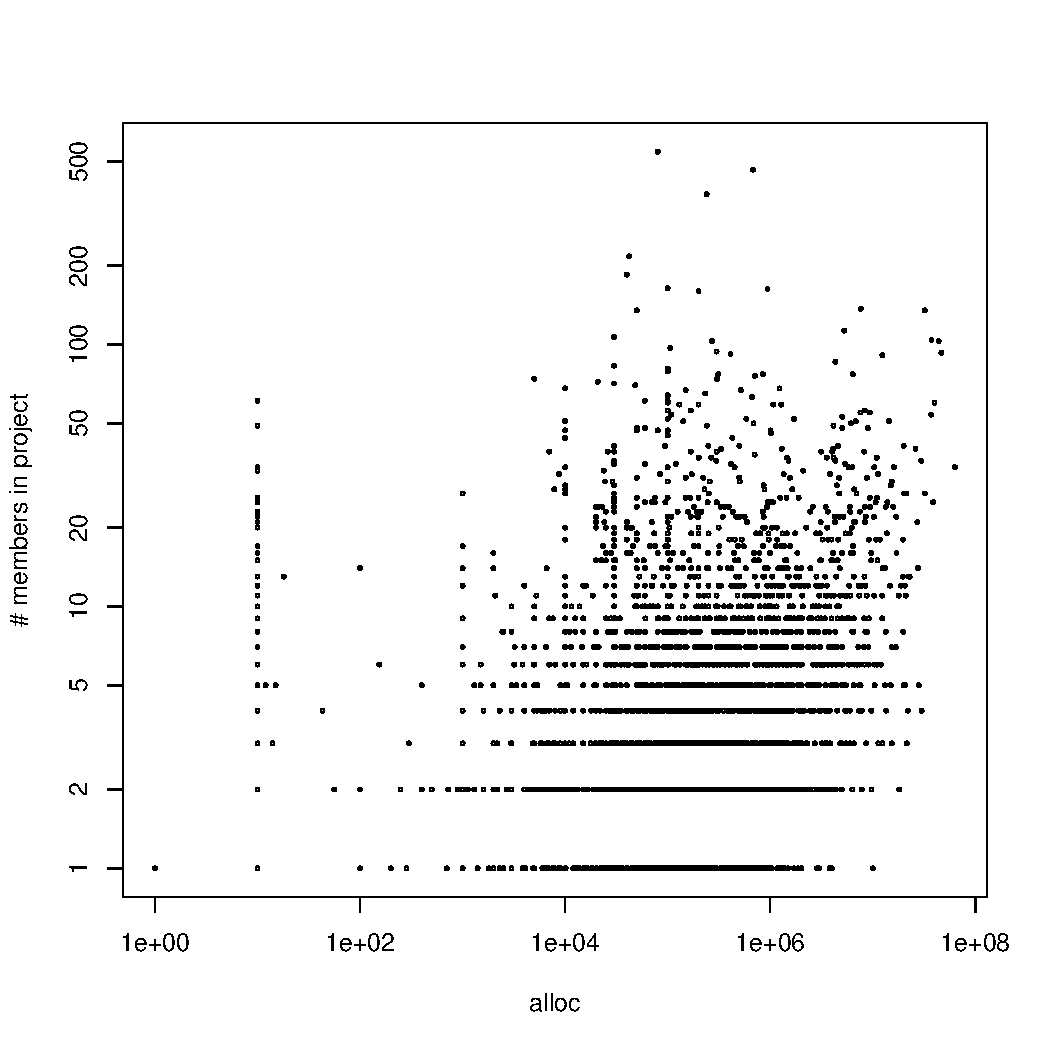
\includegraphics[width=1.0\columnwidth]{images/02_nmembers_vs_alloc_proj.pdf}
%  \caption{fig3.}\label{F:nmembers-vs-alloc-proj}
%\end{figure}

%\begin{figure}[htb]
%  \centering
%    \includegraphics[width=1.0\columnwidth]{images/05_alloc_vs_nprojects_fos_trended.pdf}
%  \caption{fig3.}\label{F:alloc-vs-nprojects-fos-trended}
%\end{figure}

%\begin{figure}[htb]
%  \centering
%    \includegraphics[width=1.0\columnwidth]{images/05_hindex_vs_nprojects_fos_trended.pdf}
%  \caption{fig3.}\label{F:hindex-vs-nprojects-fos-trended}
%\end{figure}

%\begin{figure}[htb]
%  \centering
%    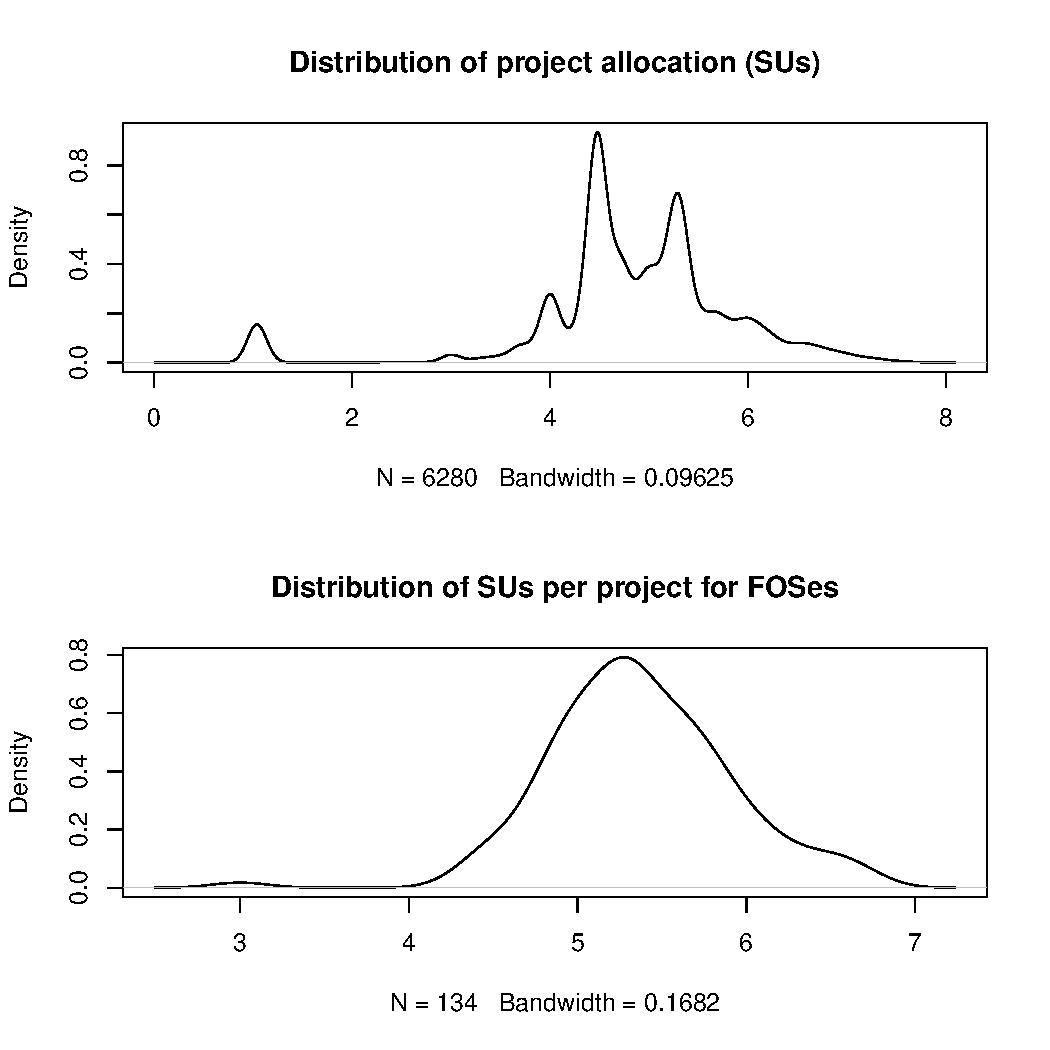
\includegraphics[width=1.0\columnwidth]{images/07_density_alloc.pdf}
%  \caption{fig3.}\label{F:density-alloc}
%\end{figure}

%\begin{figure}[htb]
%  \centering
%    \includegraphics[width=1.0\columnwidth]{images/07_density_alloc_fos_avg_by_nprojs.pdf}
%  \caption{fig3.}\label{F:density-alloc-fos-avg-by-nprojs}
%\end{figure}

%\begin{figure}[htb]
%  \centering
%    \includegraphics[width=1.0\columnwidth]{images/07_density_alloc_proj.pdf}
%  \caption{fig3.}\label{F:density-alloc-proj}
%\end{figure}


%\section{Evaluation}

\section{Conclusion}


%%%%%%%%%%%%%%%%%%%%%%%%%%%%%%%%%%%%%%%%%%%%%%%%%%%%%%%%%%%%%%%%%%%%%%
% Acknowledgment
%%%%%%%%%%%%%%%%%%%%%%%%%%%%%%%%%%%%%%%%%%%%%%%%%%%%%%%%%%%%%%%%%%%%%%

%ACKNOWLEDGMENTS are optional
%\section{Acknowledgments}

\section*{Acknowledgement}

This work is part of the Technology Auditing Service (TAS) project sponsored by NSF under grant number OCI 1025159.

\clearpage

\bibliographystyle{IEEEtranS}
%\bibliographystyle{abbrv}
\bibliography{%
%bib/references,%
%bib/vonLaszewski-jabref,%
%bib/image-refs,%
%bib/cyberaide-cloud,%
%bib/python,%
tas.bib}

\end{document}
